\documentclass[11pt]{article}

% ====================================================
% PACKAGES
% ====================================================
\usepackage[margin=1in, headheight=13.6pt]{geometry}
\usepackage[T1]{fontenc}
\usepackage{lmodern}
\usepackage{microtype}
\usepackage{setspace}
\usepackage{tcolorbox}
\usepackage{amsmath, amssymb, mathtools}
\usepackage{siunitx}

\usepackage{graphicx}
\usepackage{float}
\usepackage{subcaption}

\usepackage{enumitem}
\usepackage{booktabs}
\usepackage{longtable}
\usepackage{array}
\usepackage{multirow}

\usepackage{xcolor}
\usepackage{hyperref}

\usepackage{fancyhdr}
\usepackage{lastpage}

\usepackage{listings}
\usepackage{indentfirst}
\usepackage[justification=centering]{caption}

% Python source style for \CodeListing
\lstdefinestyle{pystyle}{
    language=Python,
    basicstyle=\ttfamily\footnotesize,
    keywordstyle=\color{blue!60!black}\bfseries,
    stringstyle=\color{orange!70!black},
    commentstyle=\color{gray!60!black}\itshape,
    numbers=left,
    numberstyle=\tiny\color{gray!70},
    numbersep=8pt,
    breaklines=true,
    showstringspaces=false,
    frame=single,
    rulecolor=\color{gray!40},
    tabsize=4,
    columns=fullflexible,
    captionpos=b,
    literate={°}{{\textdegree}}1,
}
\lstset{style=pystyle}

\pagestyle{fancy}
\fancyhf{}
\lhead{\Assignment\ |\ \course}
\rhead{\Name\ |\ \today}
\cfoot{Page \thepage\ of~\pageref{LastPage}}

\hypersetup{
    colorlinks,
    linkcolor={red!50!black},
    citecolor={blue!50!black},
    urlcolor={blue!80!black}
}

\newcommand{\Name}{Arael Anaya}
\newcommand{\Assignment}{Exam 1}
\newcommand{\course}{Advanced Dynamics}

% Boxed final-answer environment
\newtcolorbox{result}{
    colback=blue!3!white,
    colframe=blue!40!black,
    boxrule=0.6pt,
    arc=2pt,
    left=6pt, right=6pt, top=4pt, bottom=4pt
}

% Code listing: sources the .py file directly.
\newcommand{\CodeListing}[3]{%
\IfFileExists{#1}%
    {\lstinputlisting[style=pystyle,caption={#2},label={#3}]{#1}}%
    {\begin{quote}\itshape Source file \texttt{#1} not found yet --- this
        listing will populate automatically once the file is written.\end{quote}}}

\begin{document}

% ====================================================
% PROBLEM 1
% ====================================================
\section*{Problem 1}

\begin{figure}[H]
    \centering
    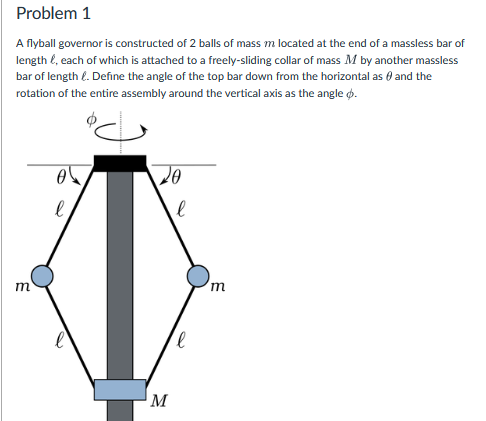
\includegraphics[width=0.7\linewidth]{Figures/Problem Set/Problem 1.png}
\end{figure}

\begin{enumerate}[label=(\alph*)]
    \item Use the vector differentiation formula to write the velocity of each particle.

    $$\hat a_1=\cos\phi\,\hat n_1+\sin\phi\,\hat n_2,\qquad \hat a_3=\hat n_3,\qquad \hat a_2=\hat a_3\times\hat a_1,\qquad {}^N\vec\omega^A=\dot\phi\,\hat n_3$$
    $$\hat e_{r_1}=\cos\theta\,\hat a_1-\sin\theta\,\hat a_3,\qquad \hat e_{\theta_1}=-\sin\theta\,\hat a_1-\cos\theta\,\hat a_3 \qquad (\text{mirrored: } \hat e_{r_2},\hat e_{\theta_2})$$
    $${}^N\vec\omega^{E_1}=\dot\phi\,\hat a_3+\dot\theta\,\hat a_2,\qquad {}^N\vec\omega^{E_2}=\dot\phi\,\hat a_3-\dot\theta\,\hat a_2$$
    $$\vec r_1=\ell\hat e_{r_1},\qquad \vec r_2=\ell\hat e_{r_2},\qquad \vec r_M=-2\ell\sin\theta\,\hat n_3$$
    \begin{align*}
    {}^N\dot{\vec r}_1 &= {}^N\vec\omega^{E_1}\times\vec r_1 = \left(\dot\phi\,\hat a_3+\dot\theta\,\hat a_2\right)\times\left(\ell\cos\theta\,\hat a_1-\ell\sin\theta\,\hat a_3\right)\\
    &= \ell\cos\theta\,\dot\phi\,\hat a_2 - \ell\cos\theta\,\dot\theta\,\hat a_3-\ell\sin\theta\,\dot\theta\,\hat a_1 = \ell\cos\theta\,\dot\phi\,\hat a_2+\ell\dot\theta\,\hat e_{\theta_1}
    \end{align*}
    $$\boxed{\vec V_1 = \ell\cos\theta\,\dot\phi\,\hat a_2+\ell\dot\theta\,\hat e_{\theta_1}} \qquad \text{(symmetry)} \qquad \boxed{\vec V_2 = -\ell\cos\theta\,\dot\phi\,\hat a_2+\ell\dot\theta\,\hat e_{\theta_2}}$$
    $$\boxed{\vec V_M = \frac{d\vec r_M}{dt} = -2\ell\cos\theta\,\dot\theta\,\hat n_3}$$

    \item What is the minimal set of generalized coordinates of the system? What is a redundant set that you could consider?

    $$\text{minimal: } \boxed{\{\theta,\ \phi\}} \qquad\qquad \text{redundant: } \boxed{\{\theta_1,\ \phi_1,\ \theta_2,\ \phi_2,\ z_M\}}$$

    \item Using the minimal set of coordinates, calculate the generalized velocity, $\dot{\vec{r}}_{ij}$, for that generalized coordinate as if you were solving this problem with D'Alembert's Principle (but don't work through the entire solution).

    $$\vec V_1 = \ell\dot\theta\,\hat e_{\theta_1}+\ell\cos\theta\,\dot\phi\,\hat a_2,\qquad \vec V_2=\ell\dot\theta\,\hat e_{\theta_2}-\ell\cos\theta\,\dot\phi\,\hat a_2,\qquad \vec V_M=-2\ell\cos\theta\,\dot\theta\,\hat n_3$$
    $$\boxed{\gamma_{1\theta}=\ell\,\hat e_{\theta_1}},\quad \boxed{\gamma_{2\theta}=\ell\,\hat e_{\theta_2}},\quad \boxed{\gamma_{M\theta}=-2\ell\cos\theta\,\hat n_3}$$
    $$\boxed{\gamma_{1\phi}=\ell\cos\theta\,\hat a_2},\quad \boxed{\gamma_{2\phi}=-\ell\cos\theta\,\hat a_2},\quad \boxed{\gamma_{M\phi}=\vec 0}$$

    \item Construct the Lagrangian and derive the equations of motion for each generalized coordinate $q_i$ of the system.

    $$|\vec V_1|^2=|\vec V_2|^2=\ell^2\dot\theta^2+\ell^2\cos^2\theta\,\dot\phi^2,\qquad |\vec V_M|^2=4\ell^2\cos^2\theta\,\dot\theta^2$$
    $$T= m\ell^2\dot\theta^2+m\ell^2\cos^2\theta\,\dot\phi^2+2M\ell^2\cos^2\theta\,\dot\theta^2, \qquad V=-2(m+M)g\ell\sin\theta$$
    $$\boxed{\mathcal L=T-V=\ell^2\left(m+2M\cos^2\theta\right)\dot\theta^2+m\ell^2\cos^2\theta\,\dot\phi^2+2(m+M)g\ell\sin\theta}$$
    \begin{align*}
    \frac{\partial\mathcal L}{\partial\dot\theta}&=2\ell^2\left(m+2M\cos^2\theta\right)\dot\theta\\
    \frac{d}{dt}\left(\frac{\partial\mathcal L}{\partial\dot\theta}\right)&=2\ell^2\left(m+2M\cos^2\theta\right)\ddot\theta-8M\ell^2\dot\theta^2\sin\theta\cos\theta\\
    \frac{\partial\mathcal L}{\partial\theta}&=-4M\ell^2\dot\theta^2\sin\theta\cos\theta-2m\ell^2\dot\phi^2\sin\theta\cos\theta+2(m+M)g\ell\cos\theta
    \end{align*}
    $$\boxed{(m+2M\cos^2\theta)\ddot\theta-2M\dot\theta^2\sin\theta\cos\theta+m\dot\phi^2\sin\theta\cos\theta-(m+M)\frac g\ell\cos\theta=0}$$
    $\phi$ cyclic ($\partial\mathcal L/\partial\phi=0$):
    $$2m\ell^2\cos^2\theta\,\ddot\phi-4m\ell^2\dot\theta\dot\phi\sin\theta\cos\theta=0 \quad\Rightarrow\quad \boxed{\ddot\phi=2\dot\theta\dot\phi\tan\theta}$$

    \item Construct the Hamiltonian of the system and write the Hamiltonian equations of motion for each generalized coordinate $q_i$ and its conjugate momentum $p_i$.

    $$p_\theta=2\ell^2(m+2M\cos^2\theta)\dot\theta,\qquad p_\phi=2m\ell^2\cos^2\theta\,\dot\phi$$
    $$\boxed{H=T+V=\frac{p_\theta^2}{4\ell^2(m+2M\cos^2\theta)}+\frac{p_\phi^2}{4m\ell^2\cos^2\theta}-2(m+M)g\ell\sin\theta}$$
    Hamilton's equations of motion:
    $$\boxed{\dot\theta=\frac{p_\theta}{2\ell^2(m+2M\cos^2\theta)}} \qquad \boxed{\dot\phi=\frac{p_\phi}{2m\ell^2\cos^2\theta}}$$
    $$\boxed{\dot p_\theta=-\frac{Mp_\theta^2\sin\theta\cos\theta}{\ell^2(m+2M\cos^2\theta)^2}-\frac{p_\phi^2\sin\theta}{2m\ell^2\cos^3\theta}+2(m+M)g\ell\cos\theta}$$
    $$\boxed{\dot p_\phi=0}$$

    \item Are there any constants of motion for this problem? List them.

    Two constants of motion:
    \begin{enumerate}[label=\arabic*.]
        \item $\boxed{p_\phi=2m\ell^2\cos^2\theta\,\dot\phi}$, the angular momentum of the two balls about the shaft axis: $\phi$ is cyclic, so no external torque acts about $\hat n_3$.
        \item $\boxed{H=E}$, the total mechanical energy: $\partial H/\partial t=0$, and therefore $H=T+V$.
    \end{enumerate}

    \item Choose your own parameters and initial conditions for the problem. Using an initial value solver, numerically integrate Hamilton's equations of motion, and plot each $q_i$, $p_i$ vs time. Additionally, plot $\theta$ vs. $\dot{\phi}$.

    Parameters: $m=1$, $M=2$, $\ell=1$; initial conditions $(\theta_0,\phi_0,p_{\theta_0},p_{\phi_0})=(0.3,\,0,\,0,\,3)$ (SI-consistent units).

    \begin{figure}[H]
        \centering
        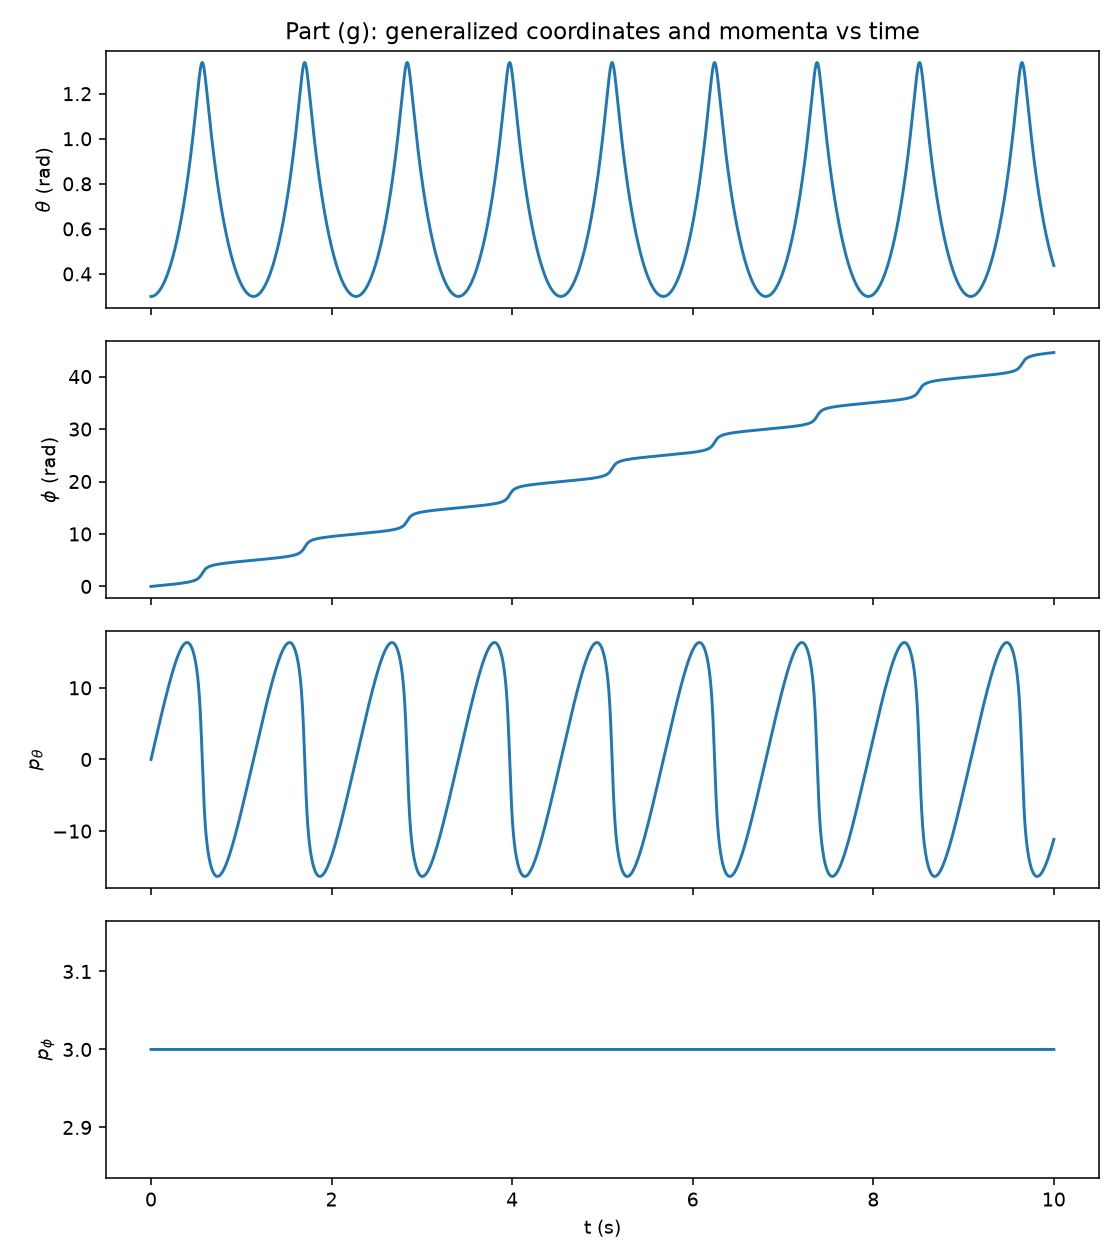
\includegraphics[width=0.75\linewidth]{Figures/Graphs/Problem1/partG_qp_vs_t.png}
        \caption{Part (g): generalized coordinates and momenta vs.\ time.}
    \end{figure}

    \begin{figure}[H]
        \centering
        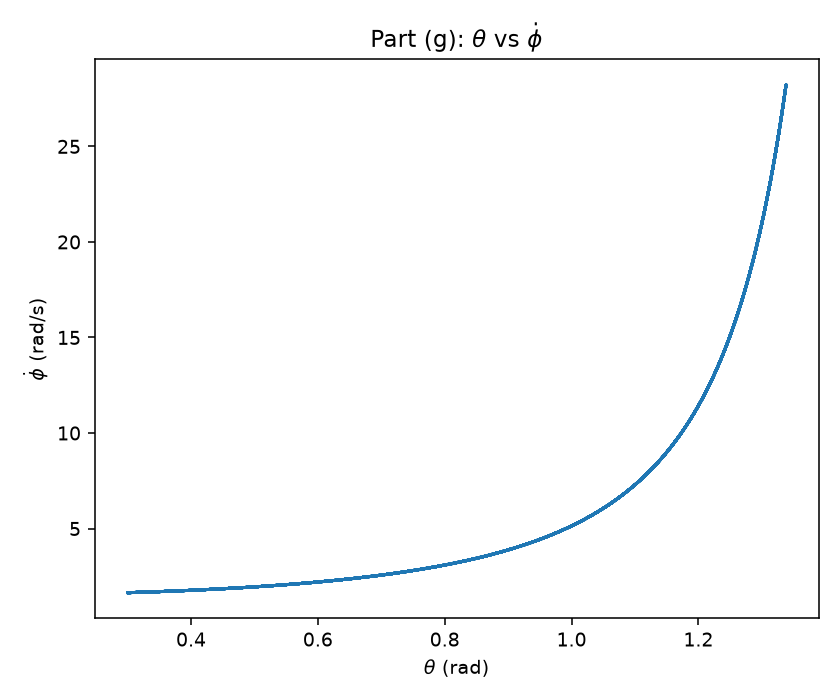
\includegraphics[width=0.75\linewidth]{Figures/Graphs/Problem1/partG_theta_vs_phidot.png}
        \caption{Part (g): $\theta$ vs.\ $\dot\phi$.}
    \end{figure}


    \item If you wanted to solve for the forces in each bar to make sure your string was strong enough, how could you solve for that?

    Newton's second law on each of the three masses gives three vector equations; the constraint force is whatever is left over once we plug in the accelerations from the Lagrangian or Hamiltonian solution. A Lagrange-multiplier approach gets there more directly, folding the bar force into the equations of motion from the start at the cost of more work.


    \item Discuss some possible approaches to the problem, including the Newtonian approach, which I didn't ask you to use here. Which approaches do you prefer? What are the different insights gained from each one?

    Any of the approaches from class would work here. Newtonian mechanics, $\vec F=m\vec a$, gets out of hand really fast with three whole particles and their constraint forces. I prefer the Lagrangian approach because everything can be put straight into the Euler--Lagrange equation. The Hamiltonian formulation splits the system into first-order equations, which is better for the numerical solver. All three, including D'Alembert's principle, discard the constraint forces along the way, so recovering them later takes extra work.

\end{enumerate}


% ====================================================
% PROBLEM 2
% ====================================================
\newpage
\section*{Problem 2}

\begin{figure}[H]
    \centering
    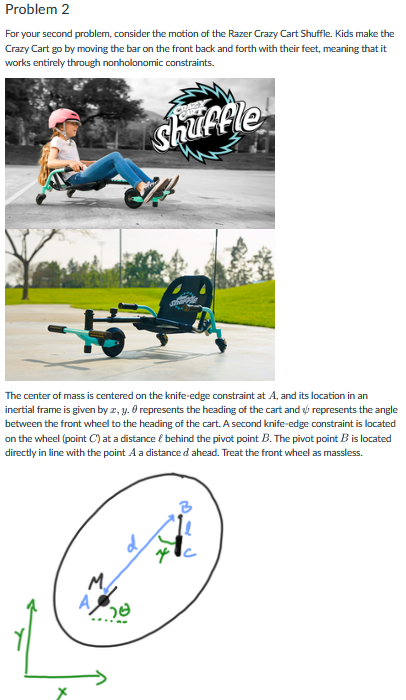
\includegraphics[width=0.7\linewidth]{Figures/Problem Set/Problem 2.png}
\end{figure}

\begin{enumerate}[label=(\alph*)]
    \item Write the two equations of constraint for the knife-edge constraints at $A$ ($\phi_1(q,\dot{q}) = 0$) and $C$ ($\phi_2(q,\dot{q}) = 0$). Hint: you may be able to use $\phi_1$ to eliminate some terms from $\phi_2$.

    $$\hat b_1=\cos\theta\,\hat n_1+\sin\theta\,\hat n_2,\quad \hat b_2=-\sin\theta\,\hat n_1+\cos\theta\,\hat n_2$$
    $$\hat c_1=\cos(\theta+\psi)\,\hat n_1+\sin(\theta+\psi)\,\hat n_2,\quad \hat c_2=-\sin(\theta+\psi)\,\hat n_1+\cos(\theta+\psi)\,\hat n_2$$

    \textbf{At $A$:} $\ {}^N\vec V_A=\dot x\,\hat n_1+\dot y\,\hat n_2$, knife edge $\Rightarrow {}^N\vec V_A\cdot\hat b_2=0$:
    $$\boxed{\phi_1=-\dot x\sin\theta+\dot y\cos\theta=0}$$

    \textbf{At $C$:} $\vec r_C=\vec r_A+d\,\hat b_1-\ell\,\hat c_1$, $\ {}^N\vec\omega^B=\dot\theta\,\hat n_3$, $\ {}^N\vec\omega^C=(\dot\theta+\dot\psi)\hat n_3$
    $$\frac{{}^Nd\hat b_1}{dt}=\dot\theta\,\hat b_2, \qquad \frac{{}^Nd\hat c_1}{dt}=(\dot\theta+\dot\psi)\,\hat c_2$$
    $${}^N\vec V_C={}^N\vec V_A+d\dot\theta\,\hat b_2-\ell(\dot\theta+\dot\psi)\,\hat c_2$$
    Knife edge $\Rightarrow \vec V_C\cdot\hat c_2=0$; using $\hat b_2\cdot\hat c_2=\cos\psi$:
    $${}^N\vec V_A\cdot\hat c_2+d\dot\theta\cos\psi-\ell(\dot\theta+\dot\psi)=0$$
    $${}^N\vec V_A\cdot\hat c_2=\cos\psi\underbrace{(-\dot x\sin\theta+\dot y\cos\theta)}_{=\ \phi_1\ =\ 0}-\sin\psi(\dot x\cos\theta+\dot y\sin\theta)=-\sin\psi(\dot x\cos\theta+\dot y\sin\theta)$$
    $$\boxed{\phi_2=-\sin\psi(\dot x\cos\theta+\dot y\sin\theta)+(d\cos\psi-\ell)\dot\theta-\ell\dot\psi=0}$$

    \item Use Lagrange's equations to derive the equations of motion for the cart in terms of Lagrange multipliers $\lambda_1$ and $\lambda_2$ corresponding to the two constraints.

    $$V=0, \qquad \mathcal L=T=\tfrac12M(\dot x^2+\dot y^2)+\tfrac12I\dot\theta^2$$
    Pfaffian form $\phi_j=\sum_i a_{ji}\dot q_i+b_j=0$, $q=(x,y,\theta)$ ($\psi(t)$ given):
    $$a_{1x}=-\sin\theta,\quad a_{1y}=\cos\theta,\quad a_{1\theta}=0$$
    $$a_{2x}=-\sin\psi\cos\theta,\quad a_{2y}=-\sin\psi\sin\theta,\quad a_{2\theta}=d\cos\psi-\ell$$
    $$\boxed{\begin{aligned}
    M\ddot x &= -\lambda_1\sin\theta-\lambda_2\sin\psi\cos\theta\\
    M\ddot y &= \lambda_1\cos\theta-\lambda_2\sin\psi\sin\theta\\
    I\ddot\theta &= \lambda_2\left(d\cos\psi-\ell\right)
    \end{aligned}}$$

    \item Solve for $\lambda_1$ and $\lambda_2$.

    Let $v\equiv{}^N\vec V_A\cdot\hat b_1$. With $\phi_1=0$: $\dot x=v\cos\theta,\ \dot y=v\sin\theta \ \Rightarrow\ {}^N\vec a_A=\dot v\,\hat b_1+v\dot\theta\,\hat b_2$.

    $$M\,{}^N\vec a_A=\lambda_1\hat b_2-\lambda_2\sin\psi\,\hat b_1 \quad\Rightarrow\quad M\dot v=-\lambda_2\sin\psi,\qquad \lambda_1=Mv\dot\theta$$
    $\phi_2=0$ in terms of $v$: $-v\sin\psi+(d\cos\psi-\ell)\dot\theta-\ell\dot\psi=0 \ \Rightarrow$
    $$\dot\theta=\frac{\ell\dot\psi+v\sin\psi}{d\cos\psi-\ell} \qquad\Rightarrow\qquad \boxed{\lambda_1=Mv\,\frac{\ell\dot\psi+v\sin\psi}{d\cos\psi-\ell}}$$
    Differentiating $\dot\theta$ and eliminating $\dot v$ via $M\dot v=-\lambda_2\sin\psi$, $\lambda_2=I\ddot\theta/(d\cos\psi-\ell)$:
    $$\ddot\theta=\frac{(d\cos\psi-\ell)(v\dot\psi\cos\psi+\ell\ddot\psi)+d\dot\psi\sin\psi(v\sin\psi+\ell\dot\psi)}{(d\cos\psi-\ell)^2+\dfrac{I}{M}\sin^2\psi} \qquad\Rightarrow\qquad \boxed{\lambda_2=\frac{I}{d\cos\psi-\ell}\,\ddot\theta}$$
    \item Assume the rider rotates the front wheel back and forth with $\psi = \frac{\pi}{6}\cos(\omega_0 t)$ rad. Plot a trajectory of $x$ vs $y$ (the motion of the center of mass) as well as $\theta$ vs $t$, given that the Crazy Cart starts at rest with $\theta_0 = 0$. You may choose your own values for mass, lengths, and moment of inertia.

    Parameters: $M=1$, $I=0.5$, $d=1$, $\ell=0.5$, $\omega_0=1$ (SI-consistent units).

    \begin{figure}[H]
        \centering
        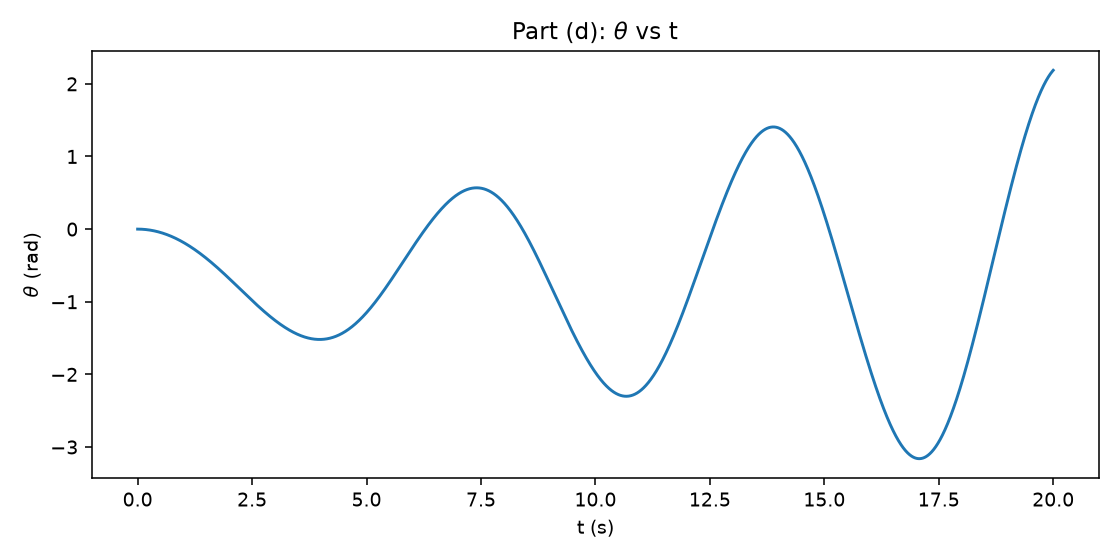
\includegraphics[width=0.75\linewidth]{Figures/Graphs/Problem2/partD_theta_vs_t.png}
        \caption{Part (d): $\theta$ vs.\ $t$.}
    \end{figure}

    \begin{figure}[H]
        \centering
        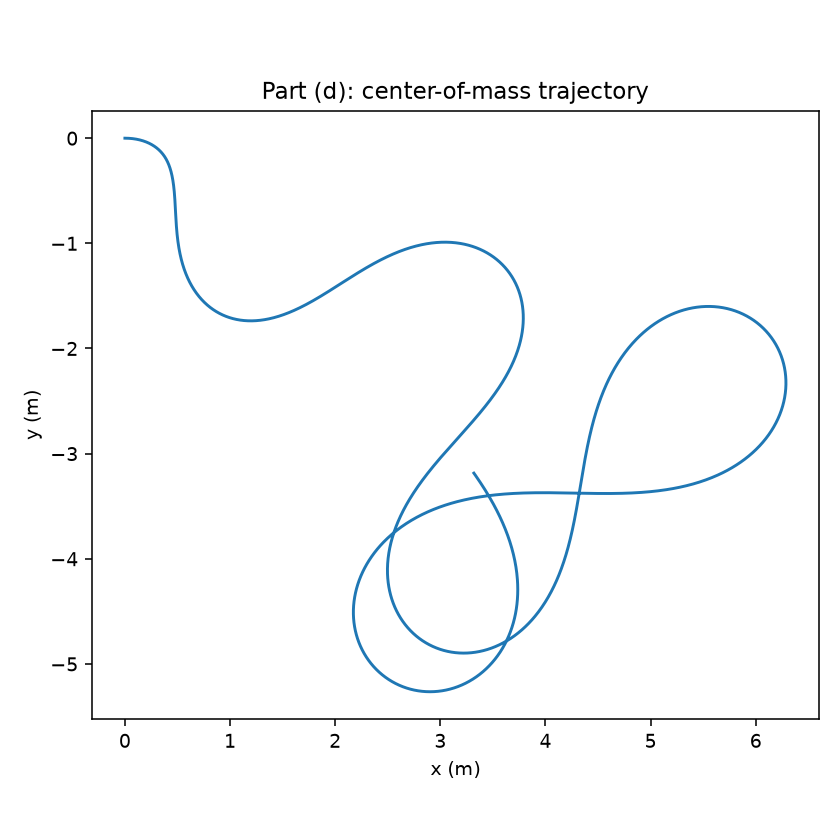
\includegraphics[width=0.7\linewidth]{Figures/Graphs/Problem2/partD_xy_trajectory.png}
        \caption{Part (d): center-of-mass trajectory under prescribed steering $\psi(t)$.}
    \end{figure}

    \item What are the key assumptions that we have made in deriving this system? What practicalities of real systems would violate these assumptions? What effect do you expect that would have on the dynamics?

    Neglecting the front wheel's mass is the biggest one. It simplifies the kinetic energy and makes the whole system driven by the prescribed steering angle $\psi(t)$: the equations never solve for $\psi$, the rider just feeds it in as a function of time. If we keep that mass term instead, and $\psi$ needs its own equation of motion, with its own inertia and angular momentum, which would couple through the constraint force $\lambda_2$ at $C$ into the cart's translational and rotational equations. The rider's steering input would then show up as a torque acting back on the cart.

    We also ignored friction and slipping at the wheels. Friction adds a non-conservative force to the energy balance. Slipping breaks the knife-edge constraints $\phi_1=0$ and $\phi_2=0$ straight up, giving the cart an extra degree of freedom in the lateral direction for as long as it lasts. The model holds only as long as the ground supplies enough friction to keep both wheels tracking. Once the wheels slip, the real motion diverges from the nonholonomic prediction.

\end{enumerate}


% ====================================================
% APPENDIX
% ====================================================
\newpage
\appendix
\section*{Appendix: Code Listings}

\subsection*{Problem 1 Code}
\CodeListing{../code/Problem1.py}{Numerical integration of Hamilton's equations of motion for the flyball governor, with an energy-conservation check.}{lst:p1}
\newpage
\subsection*{Problem 2 Code}
\CodeListing{../code/Problem2.py}{Numerical integration of the Crazy Cart's equations of motion under prescribed steering $\psi(t)$, with a constraint-satisfaction check.}{lst:p2}

\end{document}
